

\section{Singular Value Decomposition (SVD)}
We are going to use it for:
\begin{itemize}
    \item Least-squares approximation by introducing the pseudo-inverse of a matrix (Moore-Penrose inverse)
    \item Low-rank approximation with the Eckart-Young theorem
\end{itemize}
We start from:
\[
A \in \mathbb{R}^{m \times n} \hspace{1cm} 
\begin{cases}
m = \text{\# of samples}\\
n = \text{\# of features}
\end{cases}    
\]
We can write:
\[
    A = U\Sigma V^\intercal    
\]
With:
\begin{itemize}
    \item $U$ with dimensions $m \times m$ and orthogonal
    \item $\Sigma$ with dimensions $m \times n$ \textit{almost} diagonal
    \item $V^\intercal$ with dimensions $n \times n$ and orthogonal
\end{itemize}
If $m > n$, we can represent the matrices like this:
\[
\underbrace{
  \begin{bmatrix}
    & & & & & \\
    & & & & & \\
    & & & & & \\
    & & & & & \\
    & & & & & \\
  \end{bmatrix}}_{m \times m}
\underbrace{
  \begin{bmatrix}
    & & & \\
    & & & \\
    & & & \\
    & & & \\
    & & & \\
  \end{bmatrix}}_{m \times n}
\underbrace{
  \begin{bmatrix}
    & & & \\
    & & & \\
    & & & \\
  \end{bmatrix}}_{n \times n}
\]
What is the idea of SVD? Try to change features so variances are maximized and covariances are minimized. We don't want columns to be correlated.\\

In general: rank($A$) = $r < n$.
\[
    AV = U\Sigma \impliedby V^\intercal V = I \impliedby V \text{ is orthogonal}    
\]
The component wise notation is:
\[
    A\underline{v_i} = \sigma_i\underline{u_i}    
\]
Given that the rank of $A$ is $r$:

\[
\begin{bmatrix}
    & & & & & & &\\
    & & & & & & &\\
    & & & & & & &\\
    & & & & & & &\\
    & & & & & & &\\
    & & & & & & &\\
\end{bmatrix}
\begin{bmatrix}
    \sigma_1 & & & &\\
    & \sigma_2 & & &\\
    & & \ddots & &\\
    & & & \sigma_r &\\
    & & & & 0\\
    \hline
    0 & 0 & 0 & 0 & 0\\
    0 & 0 & 0 & 0 & 0\\
\end{bmatrix}
\begin{bmatrix}
    & & & & \\
    & & & & \\
    & & & & \\
    & & & & \\
\end{bmatrix}
\hspace{1cm}
\begin{cases}
\sigma_1, \dots, \sigma_r > 0\\
\sigma_{r+1}, \dots, \sigma_n = 0
\end{cases}  
\]

So the first $r$ vectors span the column space of $A$ while for the last $n-r$ means that $\underline{v_i} \in N(A)$ for $i = r+1, \dots, n$.
If we have $A^\intercal$, the decomposition is $A^\intercal = (U\Sigma V^\intercal)^\intercal = V\Sigma^\intercal U^\intercal$. 

\subsection*{Economy SVD}
What we've seen so far is the full SVD, but it can be optimized. Here is following the compact (reduced) representation, where once again we consider $m > n$:
\[
\underbrace{
  \begin{bmatrix}
    & & & \\
    & & & \\
    & & & \\
    & & & \\
    & & & \\
  \end{bmatrix}}_{m \times n}
\underbrace{
  \begin{bmatrix}
    & & & \\
    & & & \\
    & & & \\
  \end{bmatrix}}_{n \times n}
\underbrace{
  \begin{bmatrix}
    & & & \\
    & & & \\
    & & & \\
  \end{bmatrix}}_{n \times n}
\]
This is caused by the fact that the last $m-n$ rows in the central matrix are all 0 so multiply them for the last $m-n$ columns of the left matrix is useless. This can be furthermore optimized by having matrix dimensions: $(m\times r)(r\times r)(r\times n)$ because not all $\sigma$ might be different than 0 (i.e. the rank of $A$ is $r$), so, in that case is useless even to multiply the last $m-r$ rows of the central matrix. \\

\textbf{The SVD works for any matrix $A$.}\\

\noindent Let's suppose $A$ is full rank $n\times n$:
\[
    A = U\Sigma V^\intercal = \sum_{i = 1}^{n} \sigma_i \underbrace{\underline{u_i}\underline{v_i}^\intercal}_{\text{rank }=1}    
\]
If $A$ is not full rank but instead has rank($A$)=$r$, the same sum is no more computed until $n$, but instead $r$.
\[
    A = \sum_{i = 1}^{r} \sigma_i \underline{u_i}\underline{v_i}^\intercal   
\]
What happens now if we pick a certain value $\tilde{r} < r$?
\[
    A = U\Sigma V^\intercal \cong \sum_{i = 1}^{\tilde{r}} \sigma_i \underline{u_i}\underline{v_i}^\intercal   
\]
We obtain a \textbf{rank $\tilde{r}$ approximation of the matrix A}. The rank of the matrix is known because is the sum of $\tilde{r}$ matrices of rank 1. Moreover, that one, is the best approximation of rank $\tilde{r}$ possible, i.e.:
\[
    ||A - \tilde{A}|| \leq ||A - B|| \hspace{1cm} \forall B  \text{ of rank} = \tilde{r}    
\]

\subsection*{Proof that $ U\Sigma^2 U^T$ }
Once again, we start from matrix $A \in \mathbb{R}^{m \times n}$ and rank$=r$. We consider the new matrix $A^\intercal A$ which is:
\begin{itemize}
    \item symmetric: $(A^\intercal A)^\intercal = A^\intercal A$
    \item positive definite: $\underline{x}^\intercal(A^\intercal A)\underline{x} = (\underline{x}^\intercal A^\intercal)(A \underline{x}) = (A\underline{x})^\intercal (A\underline{x}) = ||A\underline{x}||^2 \geq 0  $
\end{itemize} 
We can use the following decomposition:
\[
    A^\intercal A = V\Lambda V^\intercal = \sum_{i=1}^n \lambda_i \underline{v_i} \underline{v_i^\intercal}    
\]
Recall that $V$ contains the eigenvectors while $\Lambda$ contains the eigenvalues. We rename $\lambda_i = \sigma_i^2$. The rank of $A^\intercal A$ is $r$.\\

We want to prove that if  $\underline{x} \in N(A)$ then $\underline{x} \in N(A^\intercal A)$, to do so we proceed in both directions:
\begin{enumerate}
    \item If we have $A\underline{x} = 0 \implies \underline{x} \in N(A)$. Is it possible to multiply both terms:
    \[
        A^\intercal(A\underline{x}) = A^\intercal \underline{0} = \underline{0} \hspace{1cm} \text{so} \hspace{1cm} \underline{x} \in N(A) \implies \underline{x} \in N(A^\intercal A)
    \]
    \item We start from $(A^\intercal A)\underline{x} = 0 \implies \underline{x} \in N(A^\intercal A)$. Again, we multiply:
    \[
        \underline{x}^\intercal A^\intercal A\underline{x} = ||A\underline{x}||^2 = 0 \hspace{1cm} \text{so} \hspace{1cm} \underline{x} \in N(A^\intercal A) \implies \underline{x} \in N(A)
    \]
\end{enumerate}
Let's consider the couple of (eigenvalues, eigenvectors) = ($\sigma_i^2, \underline{v_i}$):
\[
    A^\intercal A\underline{v_i} = \sigma_i^2 \underline{v_i} \hspace{0.3cm}\overset{\text{component-wise}}{\longrightarrow} \hspace{0.3cm} A^\intercal A\underline{v_i} = \sigma_i^2 \underline{v_i} \hspace{1cm} (\dagger)
\]
We introduce the quantity $\underline{u_i} = \dfrac{A\underline{v_i}}{\sigma_i}$ which has some characteristics:
\begin{enumerate}[i]
    \item $\underline{u_i}$ are unitary vectors:
    \[
        \underline{u_i}^\intercal \underline{u_i} = \left(\dfrac{A\underline{v_i}}{\sigma_i}\right)^\intercal \left(\dfrac{A\underline{v_i}}{\sigma_i}\right) = \dfrac{\underline{v_i^\intercal}A^\intercal A\underline{v_i}}{\sigma^2} \overset{\dagger}{=} \dfrac{\sigma_i^2 \underline{v_i^\intercal}\underline{v_i}}{\sigma_i^2} = 1
    \]
    The last passage of the equation is true because $\underline{v_i}$ vectors are orthonormal.
    \item $\underline{u_i} \perp \underline{u_j}$:
    \[
        \underline{u_i}^\intercal \underline{u_j} = \left(\dfrac{A\underline{v_i}}{\sigma_i}\right)^\intercal \left(\dfrac{A\underline{v_j}}{\sigma_j}\right) = \dfrac{\underline{v_i^\intercal}A^\intercal A\underline{v_j}}{\sigma_i \sigma_j} \overset{\dagger}{=} \dfrac{\sigma_j^2 \underline{v_i^\intercal}\underline{v_j}}{\sigma_i \sigma_j} = 0
    \] 
    \item $\underline{u_i}$ are eigenvectors of $AA^\intercal$ with eigenvalues $\sigma_i^2$:
    \[
        (AA^\intercal \underline{u_i}) = AA^\intercal\left(\dfrac{A\underline{v_i}}{\sigma_i}\right) = A\dfrac{A^\intercal A\underline{v_i}}{\sigma_i} \overset{\dagger}{=} A\dfrac{\sigma_i^2 \underline{v_i}}{\sigma_i} = \sigma_i^2\left(\dfrac{A\underline{v_i}}{\sigma_i}\right) = \sigma_i^2\underline{u_i}   
    \]
\end{enumerate}
We have demonstrated that $A\underline{v_i} = \sigma_i \underline{u_i}$ and $A^T\underline{u_i} = \sigma_i \underline{v_i}$ a $\underline{u_i}$ are orthonormal as well. 

We have seen that $\underline{u_i} = \frac{A\underline{v_i}}{\sigma_i}$ but, what happen if $\sigma_i = 0$?\\
Until now we have assumed that could not happen.
A concise recap of all versions of SVD:
\begin{enumerate}
    \item \textbf{full SVD}: $\underset{(m \times n)}{A} = \underset{(m \times m)}{U}\underset{(m \times n)}{\Sigma}\underset{(n \times n)}{V^\intercal}$
    \item \textbf{economy SVD}: $\underset{(m \times n)}{A} = \underset {(m \times n)}{U}\underset{(n \times n)}{\Sigma}\underset{(n \times n)}{V^\intercal}$
    \item \textbf{reduced SVD}: $\underset{(m \times n)}{A} = \underset{(m \times r)}{U}\underset{(r \times r)}{\Sigma}\underset{(r \times n)}{V^\intercal}$
    \item \textbf{truncated SVD approximation}: $\sum\limits_{i=1}^{\tilde{r}} \sigma_i\underline{u_i}\underline{v_i^\intercal}$
\end{enumerate}
For the first two cases the rank of $A$ is $n$, for the third is $r$ while in the first the approximation rank is decided.

\subsection*{Geometrical interpretation of SVD}
Matrices \( U \) and \( V^\intercal \) are orthonormal, so as mentioned in the section above, they represent rotations (or reflections), while \( \Sigma \), being a diagonal matrix, corresponds to a scaling transformation. 
\begin{center}
    \includegraphics[scale=0.4]{../images/SVD_Geometric_Interpretation.png}
\end{center}
\textbf{Since for SVD no assumptions are made on the starting matrix, this means that \underline{any} matrix can be obtained from two rotations (or reflections) and one scaling.}


For any square matrix we can apply the \textbf{polar decomposition}:
\[
A = QS
\]
where \( Q \) is orthogonal and \( S \) is symmetric positive semi-definite. Why? From SVD:
\[
    A = U\Sigma V^\intercal = \underbrace{(UV^\intercal)}_{Q} \underbrace{(V\Sigma V^\intercal)}_{S}
\]
In particular, the product of the two orthogonal matrices in the first parenthesis is always another orthogonal matrix. In this case of decomposition, matrix \( A \) is obtained just by one rotation (or reflection) and one scaling (missing one more rotation with respect to classic SVD). Indeed, the second parenthesis results in a symmetric positive semi-definite matrix because \( V \) and \( V^\intercal \) are orthogonal transformations that cancel each other out, leaving only the scaling effect from \( \Sigma \).

\subsection*{Properties of SVD}

\begin{enumerate}
    \item[i.] If \( A \) is orthogonal, then \( \sigma_i = 1 \) because if \( A \) is orthogonal, then \( A^\top A = I \).

    \item[ii.] All eigenvalues of a square matrix are \( \leq \sigma_1 \).

    \textbf{Proof:}
    \[
    \|Ax\| = \|U\Sigma V^\top x\| = \|\Sigma V^\top x\| \leq \sigma_1 \|V^\top x\| = \sigma_1 \|x\|
    \]
    
    The matrix \( U \) disappears because it is a unitary matrix, and when multiplied, it does not change the magnitude of a vector. Similarly, \( V^\top \) is also a unitary matrix, so \( \|V^\top x\| = \|x\| \).

    The inequality \( \|\Sigma V^\top x\| \leq \sigma_1 \|V^\top x\| \) holds because \( \Sigma \) is a diagonal matrix containing the singular values in descending order, with \( \sigma_1 \) being the largest. Multiplying \( \Sigma V^\top x \) scales each element of \( V^\top x \) by its corresponding singular value, and the resulting vector's norm will be less than or equal to the norm of \( V^\top x \) scaled by \( \sigma_1 \).

    \[
    \Rightarrow \|A x_i\| \leq \sigma_1 \|x_i\|
    \]

    If we consider \( \|A x_i\| = \|\lambda_i x_i\| = |\lambda_i| \cdot \|x_i\| \), then:

    \[
    |\lambda_i| \cdot \|x_i\| \leq \sigma_1 \|x_i\| \Rightarrow |\lambda_i| \leq \sigma_1 \quad \forall i
    \]
\end{enumerate}


\subsection*{Snapshots method}
During real case scenarios, we will have a certain matrix $A \in \mathbb{R}^{m\times n}$ and it might happen that $m \gg n$ i.e. the number of samples is much greater than the number of features. In these cases, we can use the following trick to be more efficient.

For the SVD we need one between  $AA^\intercal$ and $A^\intercal A$. Which one is better? And why?
We would have $AA^\intercal: (m\times m)$ and $A^\intercal A: (n\times n)$. Given $m \gg n$ it is clear that the second one is better to start with because, being much smaller, it will be easier to computer its eigenvalues and eigenvectors.    


\subsection*{Matrix norms}
This concept is an extension of the vector norm. Given a matrix $A \in \mathbb{R}^{m\times n}$, we define the matrix norm as:
\begin{itemize}
    \item \textbf{Frobenius norm}: $||A||_F = \sqrt{\sum\limits_{i=1}^{m}\sum\limits_{j=1}^{n}|a_{ij}|^2} = \sqrt{\Tr(A^\intercal A)} = \sqrt{\Tr(AA^\intercal)}$ \\
    Recall that $\Tr(AB) = \Tr(BA)$. \\

    If $U$ is orthogonal, what happen to $||AU||^2_F$?
    \[
        ||AU||^2_F = \Tr((AU)^\intercal AU) = \Tr(U^\intercal A^\intercal AU) = \Tr(A^\intercal A\underbrace{UU^\intercal}_{I}) = \Tr(A^\intercal A) = ||A||^2_F    
    \]
    This means that the Frobenius norm is invariant with respect to orthogonal transformations ($\dag$). \\ 
    The Frobenius norm is also equal to $\left(\sqrt{\sum\limits_{i=1}^{r}\sigma_i^2}\right)$ where $r$ is the rank of $A$. \\
    \textbf{Proof:}
    \[
        ||A||_F = ||U\Sigma V^\intercal||_F \overset{\dag}{=} ||\Sigma||_F \triangleq  \Tr\sqrt{(\Sigma\Sigma^\intercal)} = \sqrt{\sum\limits_{i=1}^{r}\sigma_i^2}    
    \]
    \item \textbf{P-norms}: Recall the p-norm for vectors:
    \[
        \underline{p} \in \mathbb{R}^n \implies ||\underline{p}||_p = \left(\sum\limits_{i=1}^n |p_i|^p\right)^{\frac{1}{p}}    
    \]
    Given $A \in \mathbb{R}^{m\times n}$ we can define the p-norm for that matrix as:
    \[
        ||A||_p = \underset{\underline{x} \in \mathbb{R}^n}{\sup} \dfrac{||A\underline{x}||_p}{||\underline{x}||_p} = \underset{\underline{x} \in \mathbb{R}^n, \hspace{0.1cm} ||\underline{x}||_p}{\sup} ||A\underline{x}||_p
    \]
    If you choose $p=2$ you get the operator norm and $||A||_2 = \sigma_1$.
\end{itemize}

\subsection*{Eckart-Young theorem}
Having defined the norms, we can now proceed with the proof of the \textbf{Eckart-Young theorem} which states:\\

\emph{For either $||\cdot||_F$, $||\cdot||_2$ we have:}
\[
    ||A - A_k|| \leq ||A - B|| \hspace{1cm} \forall B \text{ of rank } k
\]
\emph{where} $A_k = \sum\limits_{i=1}^k \sigma_i\underline{u_i}\underline{v_i}^\intercal$ \emph{i.e. is the SVD approximation of rank k of the matrix A. Depending on the chosen norm you get:}
\[
    ||A - A_k|| = \begin{cases}
        \sigma_{k+1} \text{ if } ||\cdot||_2 \text{considered}\\
        \left(\sum\limits_{i=1}^{r} \sigma_i^2\right)^{\frac{1}{2}} \text{ if } ||\cdot||_F \text{ considered}
    \end{cases}
\]
There will be 2 proofs, one for each type of norm. 

\subsubsection*{Proof considering $||\cdot||_F$}
We start from the \textbf{Weyl inequality}:
\[
    \sigma_{i+j-1}(X+Y) = \sigma_i(X) + \sigma_j(Y)    
\]
Where a generic $\sigma_k(E)$ is the k-eiths singular value of the matrix $E$.  
We define 
\[
X = A_k - B \hspace{2cm} Y = B    
\]
So we have
\[
\sigma_{i+k}(A) \leq \sigma_i(A-B) + \underbrace{\sigma_{k+1}(B)}_{0}
\]
The last component has value of 0 because the matrix $B$ has rank equal to $k$.
\[
||A - A_k||_F^2 = \left(\sum\limits_{i=k+1}^r \sigma_i^2(A)\right) \overset{\text{shift}}{\overset{\downarrow}{=}} \left(\sum\limits_{i=1}^{r-k} \sigma_{i+k}^2(A)\right) \leq \left(\sum\limits_{i=1}^{r-k} \sigma_{i+k}^2(A - B)\right) \leq \left(\sum\limits_{i=1}^{\min(m,n)} \sigma_{i+k}^2(A-B)\right) = ||A-B||_F^2
\]
In particular, recall that $A = \sum\limits_{i=1}^{r} \sigma_i\underline{u_i}\underline{v_i^\intercal}$ and $A_k = \sum\limits_{i=1}^{k} \sigma_i\underline{u_i}\underline{v_i^\intercal}$. The theorem is proved just by picking the first and last components of the inequality written above. 
Note that we are allowed to switch from $r-k$ to $\min(m,n)$ in the last step of the derivation of the inequality, since we are bounding from above and we are allowd to add non-negative terms on the right-hand side without affecting the inequality.
\subsubsection*{Proof considering $||\cdot||_2$}
We are now going to prove the theorem with the last norm we did not use yet. Let's consider the matrix $B$ with dimensions $n \times d$ and rank($B$)=$k$. This means that:
\[
    N(B) \subset \mathbb{R}^d \hspace{1cm} dim(N(B)) = d-k     
\]
If we consider matrix $V$ of the SVD decomposition of $A$:
\[
    V_{k+1} = \underbrace{\begin{bmatrix}
        \vline & \vline & \vline\\
        \underline{v_1} & \ldots & \underline{v_{k+1}}\\
        \vline & \vline & \vline
    \end{bmatrix}}_{k+1 \text{cols}}
\]
Those are the $k+1$ columns of $V$.
\[
\mathcal{C}(V_{k+1}) \subset \mathbb{R}^d  \hspace{1cm} dim(\mathcal{C}(V_{k+1})) = k+1  
\]
By adding the previous information, we have:
\[
    dim(N(B)) + dim(\mathcal{C}(V_{k+1})) = d - k + k + 1 = d + 1 
\]
Since both spaces are subset of $\mathbb{R}^d$ and their summed dimensions are $d+1$ this means that the intersection of those spaces is not empty.\\ 
\begin{center}
    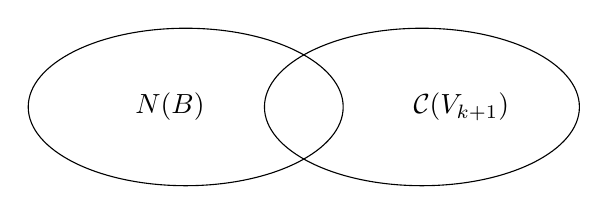
\begin{tikzpicture}
        \draw (0,0) ellipse (2cm and 1cm);
        \draw node at (-0.2,0) {$N(B)$};
        \draw (3,0) ellipse (2cm and 1cm);
        \draw node at (3.5,0) {$\mathcal{C}(V_{k+1})$};
    \end{tikzpicture}
\end{center}
Consider $\underline{w} \in N(B) \bigcap \mathcal{C}(V_{k+1})$, we suppose for easyness that $||\underline{w}||_2 = 1$.
\[
    \underline{w} = \sum_{i=1}^{k+1} c_i \underline{v_i} \overset{(\star)}{=} V_{k+1}\underline{c} \hspace{1cm} \sum_{i=1}^{k+1} c_i^2 = 1   
\]
We want to measure the following quantity:
\[
    ||A - B||^2_2 =  \underbrace{\underset{||\underline{v}||^2=1}{\sup} ||(A-B)\underline{w}||_2^2}_{\text{particular $||\underline{v}||$}} \geq \underbrace{||(A-B)\underline{w}||_2^2}_{\text{generic $||\underline{w}||$}} \implies
\]
Recall that $\underline{w} \in N(B) \implies B\underline{w} = 0$.
\[
    \implies ||A-B||^2_2 \geq ||A\underline{w}||_2^2 = \underline{w}^\intercal A^\intercal A \underline{w} \overset{\text{SVD}}{=} \underline{w}^\intercal V\Sigma^\intercal \underbrace{U^\intercal U}_{I} \Sigma V^\intercal  \underline{w} = 
\] 
\[
     \underline{w}^\intercal V\Sigma^\intercal \Sigma V^\intercal \underline{w} \overset{(\star)}{=} \underline{c}^\intercal \underbrace{V_{k+1}^\intercal V}_{I_{k+1}} \Sigma^\intercal \Sigma  \underbrace{V^\intercal V_{k+1}}_{I_{k+1}} \underline{c} = \underline{c}^\intercal \Sigma^\intercal \Sigma \underline{c} = \sum_{i=1}^{k+1} c_i^2 \sigma_i^2 \geq    
\] 
Since singular values are ordered
\[
    \geq \sigma_{k+1}^2 \underbrace{\sum_{i=1}^{k+1} c_i^2} = \sigma_{k+1}^2    
\]
So
\[
    ||A-B||_2^2 \geq \sigma_{k+1}^2 = ||A - A_k||_2^2    
\]
And, erasing the squares:
\[
    ||A - B||_2^2 \geq \sigma_{k+1} = ||A - A_k||_2        
\]
Where $A_k$ is the rank $k$ truncated SVD approximation, therefore
\[
    ||A - A_k||_2 \leq ||A - B||_2 \hspace{1cm} \forall B \text{ of rank } k
\]




